
\newpage

\section{Classification based techniques}
\label{sec:classbased}

Classification based techniques are based on systematic learning approaches based on sets of data. 
The supervised approaches require knowledge to train a model (or classifier) from a set of data instances (or training data) and classifies a new data instance as normal or as outlier. 
The unsupervised approaches do not require knowledge and learn the boundary around normal instances, declaring the new instance as normal or as outlier depending if the data instance is outside of the boundary of the previous data sets.

The classification based techniques are listed as the following:

\begin{itemize}
	\setlength\itemsep{-0.5em}
	\item Neural Networks-based;
	\item Bayesian Networks-based;
	\item Rule-based;
	\item Support Vector Machines-based.
	
\end{itemize}

\vspace{0.5em}

Neural networks-based approaches are interesting strategies for outlier detection where a given neural network might be trained with only normal data-sets. 
At testing stage, the data instances that are similar to the training data-set are accepted by the neural network and then considered as normal. 
The remaining data-sets are rejected by the neural network due to their lack of similarity with normal data-sets. Thus, those data instances are considered as outliers. 
Based on the table \ref{table:t3}, these techniques are classified as semi-supervised due to their need for normal data-sets for the training stage.

\vspace{0.5em}

Bayesian networks-based approaches are identified as prominent techniques for outlier detection in WSNs, being the reason why they are extensively covered further on in \ref{subsec:bay}.
Those techniques use probabilistic graphical models to detect outliers based on the interdependencies of different variables.

\vspace{0.5em}

Rule-based techniques, presented in \ref{subsec:rule}, classifies an outlier based on a confidence value related to the number of the training instances correctly classified by a given rule and the total number of training instances covered by the same rule. For each test instance, all the rules are tested and the confidence value is ordered. The output of this outlier detection technique is given by the inverse of the confidence value of the rule that better captures the test instance.

\vspace{0.5em}

Support Vector Machine (SVM) techniques are used for outlier detection to classify a given instance based on the fitness of a hyper-sphere to the data in a higher dimensional space. 
The hyper-sphere is obtained with a linear optimization algorithm where the objective function of this linear optimization problem is to minimize the radius R that cover the majority of the image vectors. The output of the SVM applied to OD is the classification of the image vectors as outliers if they are outside of the hyper-sphere. The SVM techniques are presented in \ref{subsec:svm}.

\newpage

\subsection{Bayesian Networks}
\label{subsec:bay}
\cite{gen:zhang:2010} divide the bayesian network based techniques in three categories: 

\begin{itemize}
	\setlength\itemsep{-0.5em}
	\item Na\"{i}ve Bayesian Networks;
	\item Bayesian Belief Networks;
	\item Dynamic Bayesian Network Models;	
\end{itemize}

All those approaches uses probabilistic graphical models to represent a set of variables and their probabilistic interdependencies. 
This graphical model aggregates the information from different variables and provides an estimate on the expectancy of an event to belong to the learned class.

\cite{class:xiang:2016} illustrates an application to measure the concentration of NO$_2$, CO and O$_3$ pollutants, using a bayesian network. All the three variables are all correlated and also depends on the temperature as presented in figure \ref{fig:xiang2016}. The real measurements acquired by the microcontroller are represented with (s) and the representations in (t) refers to the real concentration of those pollutants.

\begin{figure}[h!]
	\centering
	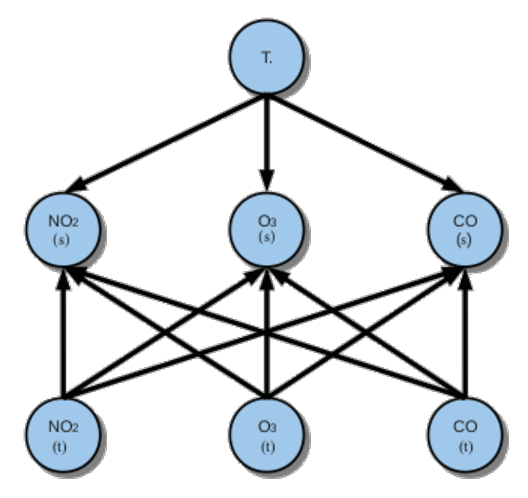
\includegraphics[width=0.60\textwidth,keepaspectratio]{figures/xiang2016}
	\caption{Application of a Bayesian Network to an atmospheric measurement system. }
	\label{fig:xiang2016}
\end{figure}

The three categories presented by \cite{gen:zhang:2010} differs between them where the first category captures the sensor nodes correlations on spatio-temporal domain; 
The second one considers not only the spatio-temporal correlations but also the conditional dependence of sensor attributes;
The third category proposes the measurement of state variables at a current time instance.

\cite{class:janakiram:2006} proposes the detection of outliers in sensor streamed data by capturing the conditional dependencies among the observation of it's attributes. this is made in three phases:

\begin{description}
	\setlength\itemsep{-0.5em}
	\item[Training Phase]  
	Phase where the Bayesian Belief Network is trained to capture the spatio-temporal correlations.
	\item[Testing Phase]  
	Phase where the trained BBN is tested on the level of accuracy and, if needed, the learned parameters are updated.
	\item[Inference Phase] 
	Phase where the missing values are inferred and the remaining streamed data are tested to detect if it is an outlier or not.
\end{description}

\cite{class:janakiram:2006} also defined the BBN, where the BBN is a directed graph, together with an associated set of probabilistic tables.
The graph is divided in nodes and arcs, where the nodes represents the variables and the arcs are the representation of the casual/influential relationship among variables.

The main contribution of BBN is the possibility to have a model that, with the dependency between uncertain variables (by filling a node probability table), it is possible to describe complex probabilistic reasoning about uncertainty.

\cite{class:janakiram:2006} describes their process in three steps:

\begin{itemize}
	%\setlength\itemsep{-0.5em}
	
	\item Constructing the Bayesian Belief Network
	\subitem \textbf{IF} a few variables have direct dependencies
	\subitem \textbf{AND} many of the variables are conditionally independent
	\subitem \textbf{THEN} all the probabilities can be computed from the joint probability distribution.
	
	\item Learning Bayesian Belief Networks
	\subitem \textbf{IF} the network structure is given
	\subitem \textbf{AND} all variables are fully observable in the training examples
	\subitem \textbf{THEN} estimating the conditional probabilities is enough
	\subitem
	\subitem \textbf{IF} the network structure is given
	\subitem \textbf{AND} some of the variables are observable
	\subitem \textbf{THEN} apply neural network using Gradient Ascent Procedure
	\subitem
	\subitem \textbf{IF} the network structure is unknown
	\subitem \textbf{THEN} Use heuristic search
	\subitem \textbf{OR} Use constraint-based technique to search through potential structures
	
	
	\item Inferring from Bayesian Belief Networks
	\subitem \textbf{THESIS} The probability distribution of certain attributes might be inferred
	\subitem \textbf{PROOF} Given the fact that the values that other attributes can take are known	
\end{itemize}

\cite{class:paola:2015} proposes an adaptive distributed Bayesian approach for detecting outliers in data collected by a WSN.
The focus of the proposed algorithm is the optimization of outlier classification accuracy, time and communication complexity and also considering externally imposed constraints on conflicting goals. The proposed algorithm is intended to run in each sensor node. 

From the individual sensor node point of view, this algorithm consists in two phases:

\begin{description}
	\setlength\itemsep{-0.5em}
	\item[Outlier detection]  
	Where, based on sensor readings and on the collaboration with neighbors, is made the probabilistic inference where the results are evaluated in three metrics: classification accuracy, time complexity and communication complexity.
	
	\item[Neighborhood selection] 
	Where the best neighbors are identified and selected to cooperate with, and, in addiction, to correspond to a reconfiguration of the Bayesian Network structure.
\end{description}

In the global point of view, if there is a high number of cooperating nodes, the classification is naturally higher with the drawback if increasing the processing time and communication complexity (thus resulting in increased detection delay and increase of energy consumption).

\cite{class:xiang:2016} proposes the addition of recover and recalibrate the drifted sensors simultaneously based on the usage of a Bayesian network. 
The authors have applied their algorithm to the measurement of the variables in the sensor readings of the NO$_2$, CO and O$_3$ pollutants, as previously presented in figure \ref{fig:xiang2016}.
Based on the correlations of the sensor readings and on the temperature influence, the algorithm itself detects the outliers, recover valid information and adjust the BBN to automatically recalibrate the sensor.




\subsection{Rule-based techniques}
\label{subsec:rule}
Rule based is another classification based technique for outlier detection. Similarly, this technique is based on a training stage from a data-set and a model generation to detect new data-instances based on history values.

Rule based techniques depends on two steps \cite{gen:chandola:2009}:

\begin{itemize}
	%\setlength\itemsep{-0.5em}
	\item \textbf{Learn rules from the training data-set}\\
	Using a learning algorithm (i.e. RIPPER, Decision Tree, etc.)\\
	Where each rule has an associated confidence value 	proportional to the ratio:\\
	{\centering	$\text{\footnotesize Confidence Value} = \frac{\text{number of training instances correctly classified by the rule}}{\text{number of total training instances covered by the rule}}$
}
		
	\item \textbf{Find for each test instance the rule}\\
	That better capture the given test instance.
	
	\item \textbf{The anomaly score is}\\
	The inverse of the confidence value for the rule that better capture the test instance.

\end{itemize}

\cite{class:islam:2016} proposes an algorithm for outlier detection inserted in rule-based taxonomy. They propose a new belief-rule-based association rule, with the focus on handling various types of uncertainties. 

Due to the nature of the sensor data, a traditional inference mechanism cannot be used. Therefore, they propose a new inference mechanism for the rule-based algorithm that consists of an input transaction database that is converted into the following:
\begin{itemize}
	\setlength\itemsep{-0.5em}
	\item belief transaction database;
	\item support calculation;
	\item belief matrix;
	\item confidence calculation;
	\item belief association rule discovery.
	
\end{itemize}


%\newpage
\vspace{1.5em}

\subsection{Support Vector Machines}
\label{subsec:svm}
Rather than performing outlier detection in the central node, \cite{class:rajasegarar:2007} proposes a 
distributed approach to:

\begin{itemize}
	\setlength\itemsep{-0.5em}
	\item performs detection on local data at each node
	\item and communicates to the parent node only the summary information to perform at upper layer the global classification of the data.	
\end{itemize}

Their proposal is based on a one-class quarter sphere SVM and is divided into 2 parts:

\begin{itemize}
	\setlength\itemsep{-0.5em}
	\item \textbf{Anomaly detection  algorithm}
	\subitem The OD is supported by previous works where, with the fitness approach of a hypersphere to the data in a higher dimensional space, and by applying a linear optimization to the problem of fitting the hypersphere with minimal radius R, having the center fixed at the origin and encompassing the majority of the image vectors.
	\subitem The result of the linear optimization problem is the classification of the image vectors as:
	
	\vspace{-1em}
	
	\subitem  \textbf{$\rightarrow$ Support Vectors}, if inside the sphere;
	\subitem  \textbf{$\rightarrow$ Outliers}, otherwise.
	\vspace{1em}
	
	\item \textbf{Distributed anomaly detection}
	\subitem \textbf{1$^{st}$ step:} Each sensor node runs the entire AD algorithm on local data;
	\subitem \textbf{2$^{nd}$ step:} The resulting radius is sent to the parent node;
	\subitem \textbf{3$^{rd}$ step:} Each parent computes the global radius;
	\subitem \textbf{4$^{th}$ step:} Parents sends the radius to children nodes;
	\subitem \textbf{5$^{th}$ step:} Children compares global radius with local one and updates parameters.
		
\end{itemize}


\cite{class:xu:2012} proposes a KNN-SVM which is a Support Vector Machine based on K-Nearest Neighbor Algorithm.

Despite KNN taxonomy is presented further on in section 3.7, in a synthesis  the KNN is a distance-based approach that detect outliers in data-instances lying in the sparsest regions or lying in the outside of a given model boundary of the feature space.

Considering the Quarter sphere SVM technique proposed by \cite{class:rajasegarar:2007} the KNN-SVM combine the origin and the radius R that contain most of the samples and introduces kernel functions to make the optimization region more tighten. 

%In two different works, \cite{class:martins:2015a} and \cite{class:martins:2015b} has proposed a modified SVM based on a kernel-based technique. In parallel, they propose an online sliding window scheme. The modification extends the original LS-SVM to be applied to the transient raw data collected from transmitters attached to a WSN. In a posterior work, \cite{class:gil:2016} compares the LS-SVM with PCA (a technique that will be presented further on in section 3.9.
\newpage





